\documentclass[12pt]{article}

\usepackage[T1]{fontenc}	%better font encoding
\usepackage[utf8]{inputenc}	%better font encoding
\usepackage{graphicx}		%allow insertion of images
\graphicspath{ {graphics/} }	% the relative path to the graphics folder
\usepackage[usenames,dvipsnames,svgnames,table]{xcolor}		%allow colour
\usepackage{amsmath,amssymb,amsthm,textcomp, xfrac}			%math symbols, etc
\usepackage{enumerate}		
\usepackage{multicol}		%allow multi columns
\usepackage{tikz}			%vector graphics
\usepackage{pgfplots}		%plots in vector graphics


%tables
\usepackage{booktabs}		%professional tables
\usepackage{tabularx, booktabs}
\newcolumntype{Y}{>{\centering\arraybackslash}X}	%type Y - even column width - centered


\usepackage{color}
\usepackage[hidelinks]{hyperref}	%hyperlinks
\hypersetup{
%    colorlinks=false, 	%set true if you want colored links
    linktoc=all,     	%set to all if you want both sections and subsections linked
%    linkcolor=blue,  	%choose some color if you want links to stand out
}

%sideways figures
\usepackage{rotating}
\usepackage{pdflscape}

%units
\usepackage{siunitx}
\usepackage{cancel}
\sisetup{load-configurations = abbreviations}
\sisetup{per-mode = symbol}

%%section style
%\usepackage{titlesec}
%\titleformat{\section}[runin]
%{\normalfont\bfseries}
%{\thesection.}{.5em}{}[]
%
%\titleformat{\subsection}[runin]
%{\normalfont\bfseries}
%{\thesubsection}{.5em}{}[]
%\setcounter{secnumdepth}{0} %dont number sections

%disable indents
%\usepackage{parskip}

%chemistry
\usepackage{mhchem}

%scientific notation  use \e
\providecommand{\e}[1]{\ensuremath{\times 10^{#1}}}

%diferential
\def \d {\ensuremath{\mathrm{d}}}

\usepackage{fullpage}		%set full page margins

\newcommand{\linia}{\rule{\linewidth}{0.5pt}}


% custom footers and headers
\usepackage{lastpage}
\usepackage{fancyhdr}
\pagestyle{fancy}
\lhead{}
\chead{}
\rhead{}
\lfoot{}
\cfoot{\thepage\ of \pageref{LastPage}}
\rfoot{}
\renewcommand{\headrulewidth}{0pt}
\renewcommand{\footrulewidth}{0pt}
%

\begin{document}

\begin{titlepage}

\newcommand{\HRule}{\rule{\linewidth}{0.5mm}} % Defines a new command for the horizontal lines, change thickness here

\center % Center everything on the page
 
%----------------------------------------------------------------------------------------
%	HEADING SECTIONS
%----------------------------------------------------------------------------------------

\textsc{\LARGE University of Victoria}\\[1cm] % Name of your university/college
\textsc{\Large ELEC 250}\\[0.5cm] % Major heading such as course name
\textsc{\large Linear Circuits: 1}\\[0.5cm] % Minor heading such as course title

%----------------------------------------------------------------------------------------
%	TITLE SECTION
%----------------------------------------------------------------------------------------

\HRule \\[0.4cm]
{ \huge \bfseries Lab 1 - Circuit Theorems}\\[0.2cm] % Title of your document
\HRule \\[1.5cm]
 
%----------------------------------------------------------------------------------------
%	AUTHOR SECTION
%----------------------------------------------------------------------------------------
%\begin{center}\large
%\emph{Instructors:} 
%\end{center}
\begin{minipage}{0.4\textwidth}
 
\begin{flushleft} \large\emph{Instructor:}
 
Dr. Nikitas \textsc{Dimopoulos} \\
\vspace{12 pt}
%\emph{Lab Supervisor:} \\
%Patrick \textsc{Chang}
\emph{Teaching Assistant:} \\
Zhen \textsc{Li}
\end{flushleft}
\end{minipage}
~
\begin{minipage}{0.4\textwidth}
\begin{flushright} \large
%Dr. Barbara \textsc{Sawicka} \\
\vspace{12 pt}
%\emph{Teaching Assistant:} \\
%Vahid \textsc{Moradi}
\end{flushright}
\end{minipage}\\[1.5cm]

% If you don't want a supervisor, uncomment the two lines below and remove the section above
\Large Clayton was here messing with things because he is a GitHub Newbie\textsc{Kihn}
\large V00794569	\\
\Large Yves \textsc{Senechal}
\large V00213837	\\
\Large Tyler \textsc{Stephen}
\large V00812021	\\
A01 - B01\\[2.5cm] % Your name

%----------------------------------------------------------------------------------------
%	DATE SECTION
%----------------------------------------------------------------------------------------

{\large \today}\\[3cm] % Date, change the \today to a set date if you want to be precise

%----------------------------------------------------------------------------------------
%	LOGO SECTION
%----------------------------------------------------------------------------------------

\includegraphics[scale=0.3]{UVic_logo}\\ % Include a department/university logo - this will require the graphicx package
 
%----------------------------------------------------------------------------------------

\vfill % Fill the rest of the page with whitespace

\end{titlepage}

\tableofcontents
\pagebreak

\section{Object}
To verify and become familiar with the following linear circuit theorems:
\begin{itemize}
	\item Kirchoff's Current and Voltage Laws
	\item Linearity and Superposition Theorems
	\item Thevenin's and Norton's Theorems
\end{itemize}
%\subsection{Objectives}
%\begin{itemize}
%\item	To learn about X-ray florescence spectroscopy through hands-on experience.
%\item	To learn the capabilities and limitations of XRF.
%\item	To learn various means of interpreting XRF data.
%\item	To learn about radioactivity, radiation sources, and radiation safety.
%\end{itemize}

%\subsection{Scope}
%The scope of the lab consisted of observing the XRF spectrometer measuring various samples and then analysing raw spectra data of a bi-metal foil and an unknown steel sample.

\section{Results}
\subsection{Kirchhoff's Current Law}
All measured current values in this section of the experiment were consistent with the calculated 
values within 5\% uncertainty. The largest source of uncertainty is the tolerance of the resistors 
(5\%). The calculated and measured quantities are summarized in Figure \ref{fig.Current} on the next page.
The consistency of the measured values with the calculations confirms that KCL can be applied 
to this circuit.

Confirmation for KCL at node A is:
\begin{center}
	$-{ I }_{ 1 }+{ I }_{ 2 }+{ I }_{ 3 }=0$\\
	$-1.4175mA\quad +\quad 0.0398mA\quad +\quad 1.4571mA\quad =\quad 79.4\mu A\quad \cong \quad 0A$\\[1em]
\end{center}

(Note: Figure 2.1 in 
the laboratory manual does not indicate any nodes. Node A has been assumed to be at the 
position directly above ${R}_{2}$ in Figure \ref{fig.setup}. However, there are no logical locations for nodes B or 
C. The upper right corner of Figure \ref{fig.setup}, where ${I}_{3}$ joins ${I}_{L}$ is a trivial node.)
\begin{figure}[htbp]
\centering
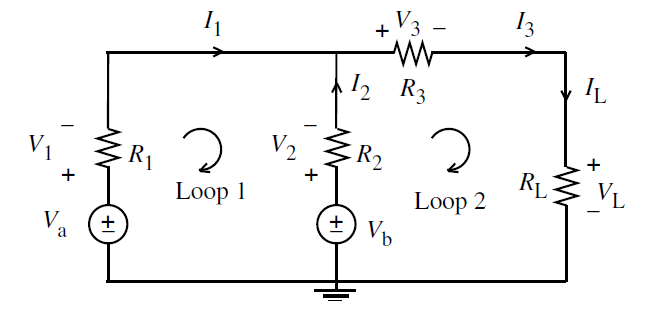
\includegraphics[scale=0.8]{Fig_2_1.png}
%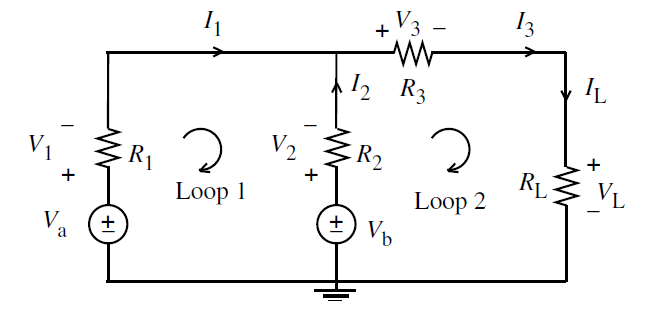
\includegraphics[scale=0.2,width=\linewidth, keepaspectratio]{Fig_2_1.png}
\caption{Initial circuit setup}
\label{fig.setup}
\end{figure}\\
\begin{figure}[htbp]
	\centering
	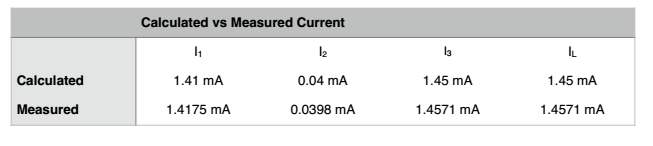
\includegraphics[scale=1]{CurrentLawMeasurement.png}
	%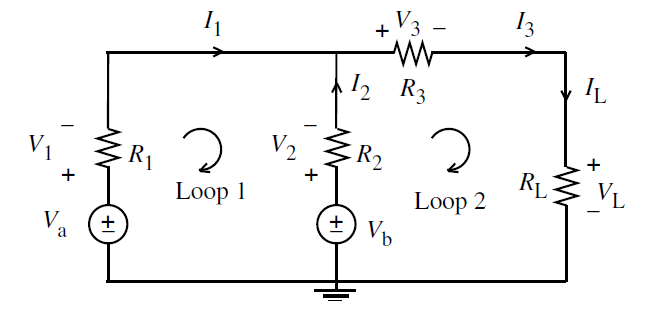
\includegraphics[scale=0.2,width=\linewidth, keepaspectratio]{Fig_2_1.png}
	\caption{Calculated current and measurement comparison}
	\label{fig.Current}
\end{figure}
%X-ray florescence spectroscopy is a non-destructive process that enables the determination of a sample's elemental composition. Both the elements present and their concentrations within the material can be ascertained. XRF can be used with a wide range of materials including: solids, liquids, organic, and inorganic objects.

%XRF involves measuring the energy of the characteristic photons that are emitted during the fluorescence process. These emitted photons take the form of unique X-rays for each element. By measuring the energy of the emitted X-rays, the element can be determined. The number of each type of emitted X-ray corresponds to the concentration of that element in the sample.

%Characteristic X-rays are emitted when the sample is illuminated with a primary beam of X or $\gamma$ rays. When these primary X-rays interact with the atoms in the sample, core electrons are ejected. As outer electrons move closer to the nucleus and fill the vacancies, the characteristic photons are emitted. 
\pagebreak

\subsection{Kirchhoff's Voltage Law}
Voltage measurements of the circuit used in 2.3.1 were consistent with the calculated values 
within 5\% uncertainty. The calculated and measured quantities are summarized in Figure \ref{fig.Voltage}.
The consistency of the measured values with the calculations confirms that KVL can be applied 
to this circuit.
Confirmation of KVL in loops 1 and 2 are:

\begin{center}
	$-{ V }_{ a }+{ V }_{ 1 }-{ V }_{ 2 }+{ V }_{ b }=0\quad (loop 1)$\\
	$-6.0306V+3.1098V-0.0869V+2.9839V\quad =\quad -0.0238V\quad \cong \quad 0V$\\[1em]
\end{center}

\begin{center}
	$-{ V }_{ b }+{ V }_{ 2 }+{ V }_{ 3 }+{ V }_{ L }=0\quad (loop 2)$\\
	$-2.9839V+0.0869V+1.4493V+1.4460V\quad =\quad -0.0017V\quad \cong \quad 0V$\\[1em]
\end{center}

\begin{figure}[htbp]
	\centering
	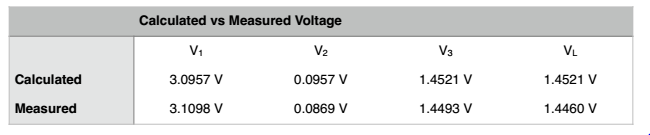
\includegraphics[scale=1]{VoltageLawMeasurement.png}
	%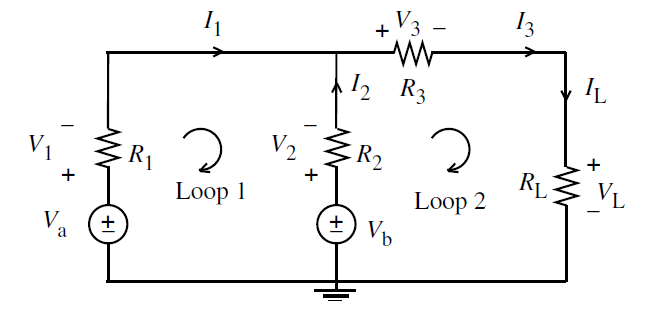
\includegraphics[scale=0.2,width=\linewidth, keepaspectratio]{Fig_2_1.png}
	\caption{Calculated voltage and measurement comparison}
	\label{fig.Voltage}
\end{figure}
\pagebreak
%The equipment used in the lab was an industrial-type hand-held XRF spectrometer type XMET920. Spectra data was graphed and analysed using Microsoft Excel.

\subsection{Linearity Theorem}
The first step in this section was to disable the voltage source $ V_{b}$ of Figure \ref{fig.setup} by replacing it with a short circuit. The input voltage source $V_{a}$ was then varied to obtain the load current and load voltage plots of Figures \ref{fig.CurrentLinearity} and \ref{fig.Voltagelinearity} below.\\
\begin{figure}[htbp]
	\centering
	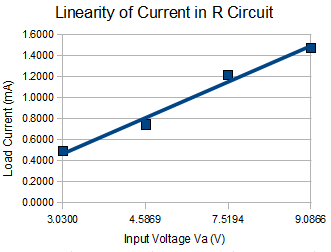
\includegraphics[scale=1]{CurrentLinearity.png}
	%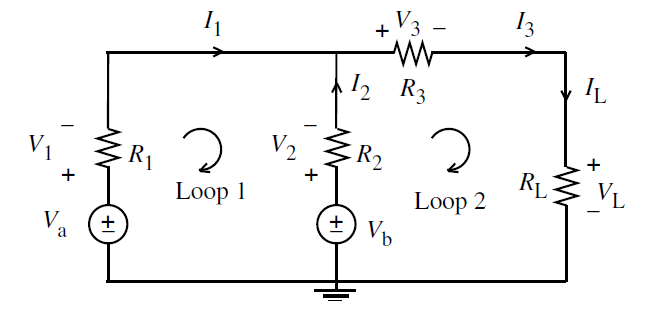
\includegraphics[scale=0.2,width=\linewidth, keepaspectratio]{Fig_2_1.png}
	\caption{Linearity of Resistive Circuit}
	\label{fig.CurrentLinearity}
\end{figure}\\
\begin{figure}[htbp]
	\centering
	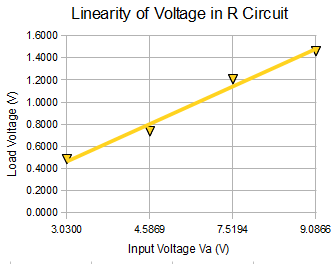
\includegraphics[scale=1]{VoltageLinearity.png}
	%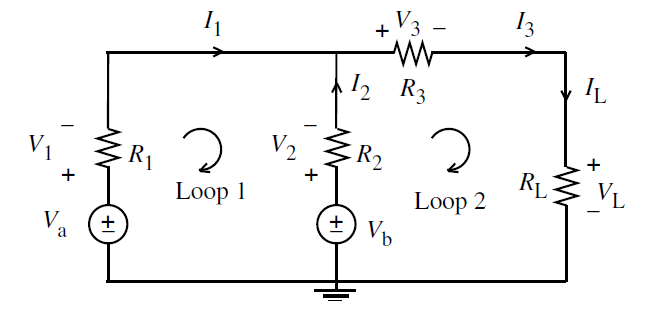
\includegraphics[scale=0.2,width=\linewidth, keepaspectratio]{Fig_2_1.png}
	\caption{Linearity of Resistive Circuit}
	\label{fig.Voltagelinearity}
\end{figure}\\
\pagebreak
\vfill
The theoretical proportionality constants for this modified circuit were calculated using the following equations:
\begin{center}
	$V_{L} = K_{1}V_{a}$\\
	$I_{L} = K_{2}V_{a}$\\[1em]
	Where $K_{1} =\frac{0.970}{6} = 0.162$,\\[0.3em]
	and $K_{2} = \frac{0.970}{6} = 0.162$
\end{center}
The experimental proportionality constants using meter readings were as follows:

\begin{center}
	$K_{1} =\frac{1.4616}{9.0866} = 0.1609$,\\[0.3em]
	and $K_{2} = \frac{1.4729}{9.0866} = 0.1621$
\end{center}
Thus, the theoretical and experimental proportionality constants agree to two decimal places.
\begin{figure}[htbp]
	\centering
	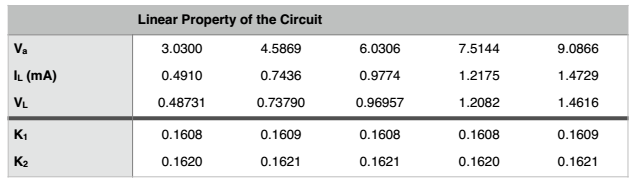
\includegraphics[scale=1]{LinearityMeasurement.png}
	%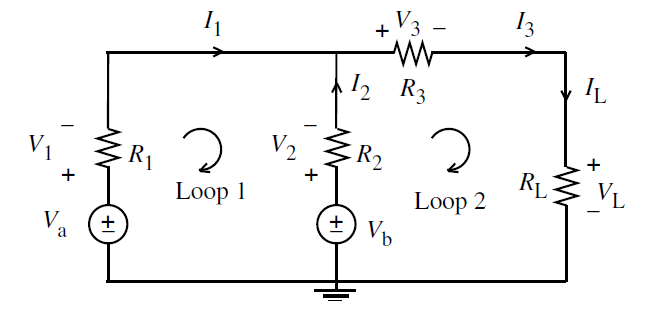
\includegraphics[scale=0.2,width=\linewidth, keepaspectratio]{Fig_2_1.png}
	\caption{Linearity}
	\label{fig.linMeasure}
\end{figure}
%Prior to the XRF measurement, the spectrometer must be calibrated and the input variables set. These variables include: geometry, measurement time, primary radiation source, and data evaluation mode. The actual XRF measurement is automatic and controlled by the computer. After the measurement is complete the data can be automatically analysed by the computer,the generated spectra can be viewed, or the data can be saved for further analysis.
\pagebreak
\subsection{Superposition Theorem}
In this section, the circuit is still configured as in the previous step with $V_{a}$ set to 6 V. The load voltage and current were then measured to be 0.96957 V and 0.9774 mA respectively. These figures closely agreed with the theoretically calculated values of 0.97 V and 0.970 mA. The next circuit modification was to disable $V_{a}$ and reconnect $V_{b}$ with a voltage of 3 V. This time, the load voltage and current were measured to be 0.4804 V and 0.4841 mA. The theoretical values were 0.484 V and 0.484 mA. Again, the measurements and theoretical values agree to 2 decimal places.\\
From sections 2.3.1 and 2.3.2 in the lab manual, the values of $V_{L}$ and $I_{L}$ were found to be 1.4460 V and 1.4571 mA. Using these values and measurements from this section we were able to verify the superposition theorem which states:
\begin{center}
	$V_{L} = V_{La}+V_{Lb}$\\
	$I_{L} = I_{La}+I_{Lb}$
\end{center}
From our measurements we obtained:
\begin{center}
$0.96957 V + 0.4804 V = 1.4500 V$\\
$0.9774 mA + 0.4841 mA = 1.4615 mA$	
\end{center}
Both values agree to theoretical values by at least one decimal place and verify the superposition theorem.
\begin{figure}[htbp]
	\centering
	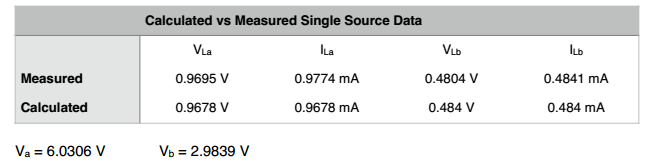
\includegraphics[scale=1]{SuperpositionMeasurement.png}
	%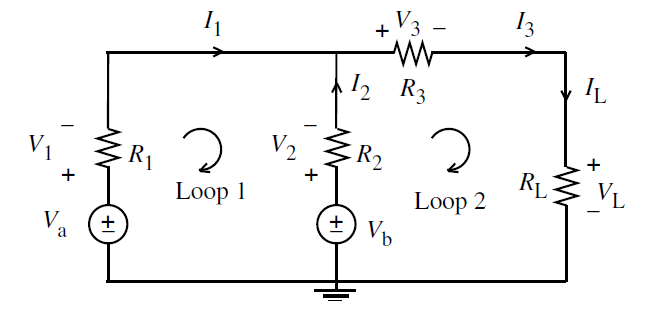
\includegraphics[scale=0.2,width=\linewidth, keepaspectratio]{Fig_2_1.png}
	\caption{Superposition Measurements}
	\label{fig.superMeasure}
\end{figure}
\pagebreak
\subsection{Thevenin's Theorem}
To calculate Thevenin’s equivalent, the circuit was configured as in Figure 1 with the exception of resistor RL which was disconnected. The potential difference across AB ($V_{ab}$) was measured to be $V_{ab}$= 4.5051 V, where $V_{ab}$ = $V_{T}$ and $V_{T}$ is the Thevenin equivalent voltage.

With resistor $R_{L}$ still disconnected and $V_{a}$ and $V_{b}$ disabled, the equivalent circuit resistance was measured to be $R_{T}$ = 2.0847k$\Omega$, where $R_{T}$ is the Thevenin equivalent resistor. The measured $R_{T}$ was within the 5\% uncertainty of the calculated 2.11 k$\Omega$.

The circuit was then reconfigured to replicate Figure \ref{fig.Thevenin} with $V_{T}$ = 4.5051 V, and $R_{T}$ = 2.0707 k$\Omega$ +/- 5\%. Two 1 k$\Omega$ and one 100 $\Omega$  resistors in series were chosen to replicate this circuit. In this configuration, $V_{L}\prime$ and $I_{L}\prime$ were measured to be 1.4486 V and 1.4613 mA respectively, which were within 5\% uncertainty of the $V_{L}$ and $I_{L}$ (1.4460 V and 1.4571 mA) measured in section 2.3.1 and 2.3.2.
\begin{figure}[htbp]
	\centering
	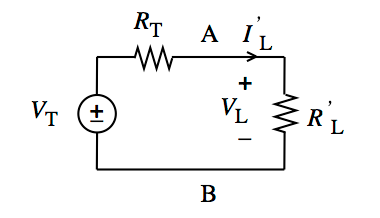
\includegraphics[scale=.65]{Thevenin.png}
	%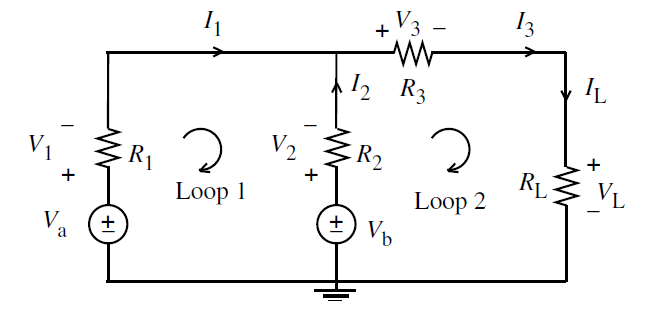
\includegraphics[scale=0.2,width=\linewidth, keepaspectratio]{Fig_2_1.png}
	\caption{Thevenin Equivalent}
	\label{fig.Thevenin}
\end{figure}
\begin{figure}[htbp]
	\centering
	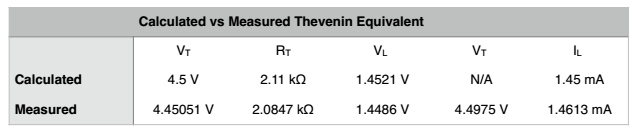
\includegraphics[scale=1]{TheveninMeasurement.png}
	%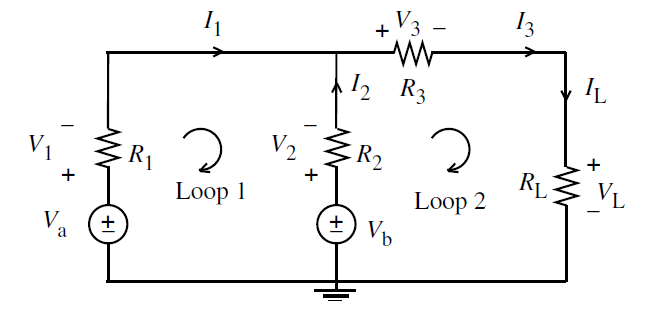
\includegraphics[scale=0.2,width=\linewidth, keepaspectratio]{Fig_2_1.png}
	\caption{Thevenin Measurements}
	\label{fig.TheveninMeasure}
\end{figure}
\pagebreak
\subsection{Norton's Theorem}
To calculate Norton’s equivalent, the circuit was configured as in Figure 1 with the exception of $R_{L}$ being replaced with a short-circuit. The current $I_{N}$ (Norton equivalent) across the short-circuit was measured to be 2.1511 mA. The circuit was then reconfigured to replicate Figure \ref{fig.NortonEquivalent} with $I_{N}$ = 2.1511mA and $R_{T}$ = 2.0707 k$\Omega$ +/- 5\% (from 2.3.5). In this circuit configuration, $V_{L}\prime\prime$ and $I_{L}\prime\prime$ were measured to be 1.4747 V and 1.4767 mA respectively, which is within 5\% uncertainty of the $V_{L}$ and $R_{L}$ (1.4460 V and 1.4571 mA) measured in section 2.3.1 and 2.3.2.
\begin{figure}[htbp]
	\centering
	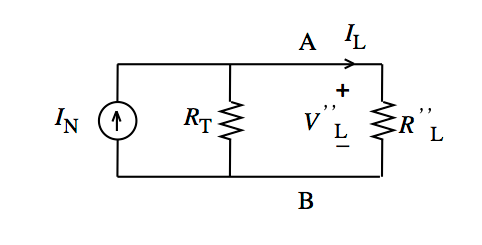
\includegraphics[scale=.65]{Norton.png}
	%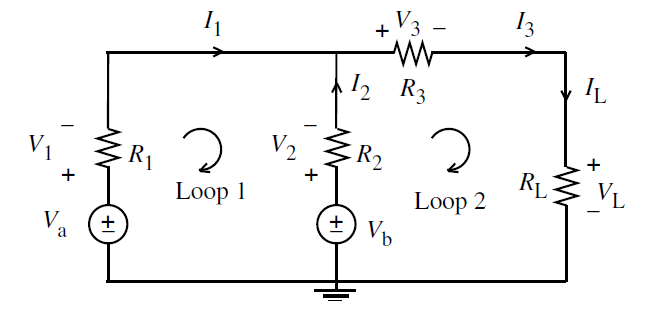
\includegraphics[scale=0.2,width=\linewidth, keepaspectratio]{Fig_2_1.png}
	\caption{Norton Equivalent}
	\label{fig.NortonEquivalent}
\end{figure}

Norton’s theorem, which states that a single current source and resistor in parallel can represent a more complex circuit, has been verified experimentally. The circuits from Figure \ref{fig.setup} and Figure \ref{fig.NortonEquivalent} are completely different, yet they yield the same results regarding voltage and current across the load resistor ($R_{L}$).
\begin{figure}[htbp]
	\centering
	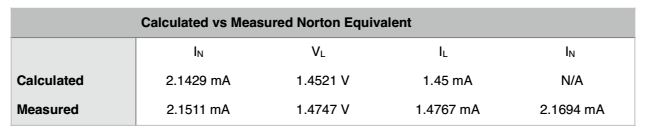
\includegraphics[scale=1]{NortonMeasurement.png}
	%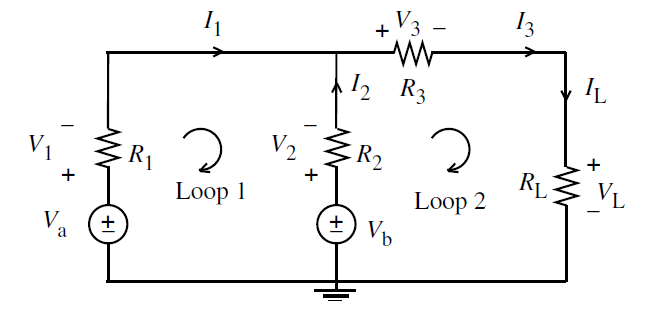
\includegraphics[scale=0.2,width=\linewidth, keepaspectratio]{Fig_2_1.png}
	\caption{Norton Measurements}
	\label{fig.Norton}
\end{figure}
%\section{Discussion and Conclusions}
\section{Attachments}
\subsection{Measurements}
\subsection{Prelab Work}
%\subsection{Measurements}
%\subsection{Foil Composition} \label{sec.foilcomposition}
%The XRF spectra of samples ASAND3 and ASAND4 are shown in figure \ref{fig.bimetal}. These samples are both sides of a bi-metal foil. The values of the energy peaks, the associated element, and x-ray lines are shown in table \ref{tab.bimetal_peaks}. As shown in figure \ref{fig.bimetal} and table \ref{tab.bimetal_peaks}, both samples contain zirconium and niobium. However, the number of counts vary between the samples; ASAND3 has higher counts for the niobium k-lines, while ASAND4 has higher counts for the zirconium k-lines. This indicates that the bi-metal foil is a sandwich of two distinct layers, as opposed to an alloy of the two metals. If each side of the sample displayed an identical spectra, the specimen would be an alloy.

% Table generated by Excel2LaTeX from sheet 'Sheet1'
%\begin{table}[htbp]
 % \centering
  %\caption{Energy peaks of figure \ref{fig.bimetal}.}
   % \begin{tabular}{ccc}
   % \toprule
   % Energy Peak (keV) & Element & Emitted X-Ray Line \\
   % \midrule
    %15.7  & Zirconium  & K$_\alpha$ \\
    %16.5  & Niobium & K$_\alpha$ \\
    %17.6  & Zirconium  & K$_\beta$ \\
    %18.6  & Niobium & K$_\beta$ \\
    %\bottomrule
    %\end{tabular}%
  %\label{tab.bimetal_peaks}%
%\end{table}%



%\subsection{Number of Measurements} %\label{sec.number_of_measurements}
%If only one measurement was taken there would be insufficient information to determine the nature of the foil. One measurement can show that there are two elements present, what elements they are, and what their relative quantities are; however it can not reveal any information about the structure of the sample. For example, a single spectra showing the two elements could be an evenly distributed alloy, or multiple distinct layers of the two metals. If the only possible configurations are an alloy or a two layer sandwich, then a measurement of each side is sufficient to determine the structure of the specimen. However, if there are other possible configurations, such as the previously mentioned multiple distinct layers, or regions of varying concentration, two samples would be insufficient to determine the structure.

%\begin{landscape}
%\begin{figure}[htbp]
%\centering
%\includegraphics[width=\linewidth, keepaspectratio]{Task2.pdf}
%\caption{XRF spectra of both sides of a bi-metal foil.}
%\label{fig.bimetal}
%\end{figure}
%\end{landscape}

%\subsection{Thickness Estimation} \label{sec.foil_thickness}
%The relative K$_\alpha$ line amplitudes of the spectra are shown more clearly in figure \ref{fig.bimetal_heights} and compared in table \ref{tab.bimetal_thick}. These amplitudes reveal additional information about the structure of the bi-metal foil. ASAND4 has a higher zirconium peak than ASAND3, indicating that measurement ASAND3 was of the niobium side of the foil while ASAND4 was of the zirconium side. Even though the peak hight values have not been corrected, they allow a rough quantitative evaluation of the concentration of each element. As zirconium and niobium are adjacent in the periodic table, the $\tau$ and $\omega$ correction coefficients would be similar, due to the closeness of the elements' spectral lines and the minor difference in atomic number, respectively. 

%\begin{table}[htbp]
 % \centering
  %\caption{Rough evaluation of bi-metal foil elemental thickness.}
   % \begin{tabular}{ccccc}
    %\toprule
     %Element     & \multicolumn{2}{c}{{K$_\alpha$ Peak Height (counts)}} &   Ratio    &  Estimated Thickness \\
    %\cmidrule(lr){2-3}
     %& ASAND3 & ASAND4 &  (ASAND3:ASAND4) & (mm) \\
    %\midrule
    %Zr    & 11900 & 64300 & 18.5\% & 0.04 \\
    %Nb    & 31000 & 45200 & 68.6\% & 0.1 \\
    %\bottomrule
    %\end{tabular}%
 % \label{tab.bimetal_thick}%
%\end{table}%


%Table \ref{tab.bimetal_thick} also shows the ratio between the K$_\alpha$ peak heights for each metal. This indicates that the niobium layer absorbed approximately 80\% of the emitted zirconium photons in the ASAND3 sample and the zirconium layer absorbed approximately 30\% of the emitted niobium photons in the ASAND4 sample. This indicates that the niobium layer is thicker than the zirconium layer. When these absorption values are compared against the ten-value layer data for zirconium at 15 keV (shown in table \ref{tab.zr15kev_absorption}) the thickness of each layer can be estimated. The zirconium ten-value layer data at 15 keV is used for both the zirconium and niobium thickness estimation as it is closest in energy and atomic number. The zirconium layer is approximately \SI{0.04}{mm} and the niobium layer is approximately \SI{0.1}{mm}. Additionally, the low level of backscattering radiation seen in figure \ref{fig.bimetal} indicates a thicker sample capable of blocking the detector from most of the primary radiation reflecting off surroundings.

% Table generated by Excel2LaTeX from sheet 'Sheet2'
%\begin{table}[htbp]
 % \centering
  %\caption{Zirconium X-ray absorption at 15 keV.}
   % \begin{tabular}{cc}
    %\toprule
    %Absorption & Thickness (mm) \\
    %\midrule
    %99\%  & 0.288 \\
    %90\%  & 0.144 \\
    %50\%  & 0.043 \\
    %\bottomrule
    %\end{tabular}%
  %\label{tab.zr15kev_absorption}%
%\end{table}%

%\begin{figure}[htbp]
%\centering
%\includegraphics{Task2_peakheight.pdf}
%\caption{Enhanced area of XRF spectra of bi-metal foil showing K$_\alpha$ peak heights.}
%\label{fig.bimetal_heights}
%\end{figure}



%\section{Steel Identification}



%\subsection{Alloy Elements} % \label{sec.steel_alloyelements}
%The XRF spectra of steel samples S1 and S22 are shown in figure \ref{fig.steel}. An enhanced area of these spectra is shown in figure \ref{fig.steel_zoom}. Sample S1 is essentially pure iron while sample S22 is an unknown grade of steel with various alloying elements. The values of the energy peaks, the associated alloying element, and x-ray lines of sample S22 are shown in table \ref{tab.steel_peaks}.

%\begin{landscape}
%\begin{figure}
%\centering
%\includegraphics[width=\linewidth, keepaspectratio]{Task3.pdf}
%\caption{XRF spectra of two steel samples.}
%\label{fig.steel}
%\end{figure}
%\end{landscape}

% Table generated by Excel2LaTeX from sheet 'Sheet1'
%\begin{table}[htbp]
 % \centering
  %\caption{Energy peaks of steel sample S22 from figures \ref{fig.steel} and \ref{fig.steel_zoom}.}
   % \begin{tabular}{ccc}
    %\toprule
    %Energy Peak (keV) & Corresponding Element & Wave Function \\
    %\midrule
    %4.7   & Titanium & K$_\alpha$ \\
    %4.9   & Vanadium & K$_\alpha$ \\
    %5.4   & Chromium & K$_\alpha$ \\
    %6.4   & Iron  & K$_\alpha$ \\
    %7.1   & Iron  & K$_\beta$ \\
    %8.4   & Tungsten  & L$_\alpha$ \\
    %9.7   & Tungsten & L$_\beta$ \\
    %11.3  & Tungsten & L$_\gamma$ \\
    %17.5  & Molybdenum & K$_\alpha$ \\
    %\bottomrule
    %\end{tabular}%
  %\label{tab.steel_peaks}%
%\end{table}%

%\begin{figure}[htbp]
%\centering
%\includegraphics[width= \textwidth]{Task3_Zoom.pdf}
%\caption{Enhanced area of XRF spectra of two steel samples.}
%\label{fig.steel_zoom}
%\end{figure}






%\subsection{Rough Evaluation of Alloy Concentrations} \label{sec.steel_roughconcentations}
%Table \ref{tab.steel_height} shows the peak heights of the alloying elements from sample S22. These values give a very rough indication of the concentration of each alloying element in the steel sample. However, the large range in atomic number and energy of the characteristic x-rays among these elements affects the accuracy of the information. To obtain more accurate concentration data these values must be adjusted by using $\tau$ and $\omega$ correction coefficients. The correction factor and adjusted peak hight values are also shown in table \ref{tab.steel_height}. These corrected values are still not entirely accurate as the matrix absorption affects have not be accounted for, though they should help to narrow the determination of the steel grade.

% Table generated by Excel2LaTeX from sheet 'Sheet1'
%\begin{table}[htbp]
 % \centering
  %\caption{Raw and corrected peak heights of S22 alloying elements.}
   % \begin{tabular}{cccc}
   % \toprule
%    Element & Peak Height (counts) & Correction Factor & Corrected Height (counts) \\
    %\midrule
%    Titanium    & 30    & 200\% & 60 \\
    %Vanadium     & 90    & 200\% & 180 \\
    %Chromium    & 810   & 200\% & 1620 \\
    %Tungsten     & 1630  & 115\% & 1870 \\
    %Molybdenum    & 630   & 30\% & 190 \\
    %\bottomrule
    %\end{tabular}%
  %\label{tab.steel_height}%
%\end{table}%

%\subsection{Identification using Alloy Concentrations} \label{sec.steel_ID_with_heights}
%By comparing the corrected peak heights from table \ref{tab.steel_height}, ratios can be determined between the alloying elements. These ratios can then be compared against known steel grade standards to determine the grade of the unknown sample. Table \ref{tab.steel_height} shows that the primary alloying elements are tungsten and chromium in roughly equal parts followed by vanadium and molybdenum again in roughly equal quantities. The ratio between tungsten/chromium and vanadium/molybdenum is roughly 10:1. 
%Two standard grades of steel IARM-44A and IARM-48A both contain large quantities of tungsten and chromium, as seen in table \ref{tab.steel_grades}. The ratio between tungsten and chromium in IARM-44A is very close to that of the unknown sample S22, but this steel also has large quantities of molybdenum which are not seen in S22. IARM-48A contains larger quantities of tungsten and chromium than vanadium and molybdenum, but the tungsten/chromium ratio is much higher than that in S22. Using only the data from table \ref{tab.steel_height} it is difficult to determine the identity of sample S22, as it bears similarity to both IARM-44A and IARM-48A.

% Table generated by Excel2LaTeX from sheet 'Sheet2'
%\begin{table}[htbp]
%  \centering
%  \caption{Major alloying elements in two steel grades.}
 %   \begin{tabular}{ccccccccccccc}
  %  \toprule
   % 	QA\# 	&	Grade	& \multicolumn{9}{c}{{Alloying Element Weight Percentage}}	\\
    %\cmidrule(lr){3-11}
    %	&		& V& Cr &Mn &Fe &Ni& Mo& W & Sn & Cu \\
    %\midrule
   % IARM-44A &Tool steel M2 &1.86 &4.26 &0.31 &80.39& 0.2& 5.08 &6.25 & 0.011 & 0.14 \\
    %IARM-48A &Tool steel T1 &1.13 &4.32 &0.33 &73.89 &0.23 &0.4 &17.99 & 0.019 & 0.13 \\
    %\bottomrule
    %\end{tabular}%
  %\label{tab.steel_grades}%
%\end{table}%

%\subsection{Identification using Analysing Model} \label{sec.steel_modelanalysis}
%The results of semi-empirical computer analysis of sample S22 are shown in table \ref{tab.steel_computermodel}. When these results are compared aginst the two likely candidates in table \ref{tab.steel_grades}, it becomes clear that sample S22 most closely matches the  IARM-48A profile. The very high tungsten content is the deciding factor.

% Table generated by Excel2LaTeX from sheet 'Sheet2'
%\begin{table}[htbp]
 % \centering
  %\caption{Semi-empirical analysis of sample S22 using computer modelling.}
   % \begin{tabular}{*{8}{c}}
    %\toprule
    %Sample & \multicolumn{7}{c}{{Alloying Element Weight Percentage}} \\
    %\cmidrule(lr){2-8}
    %& V & Cr & Mn & Ni & Cu & Mo & W \\
    %\midrule
    %S22 & 0.06 & 2.4 & 0.00 & 0.00 & 0.00 & 0.27 & 17.9 \\
    %\bottomrule
    %\end{tabular}%
  %\label{tab.steel_computermodel}%
%\end{table}%

%\subsection{Merits of Identification Methods}
%Both methods of spectra analysis are useful in determining the contents and concentrations of an unknown sample. The semi-empirical computer analysis is quicker and more accurate, but has a few limitations. The analysis is only as good as the model, and the model must have some resemblance to the unknown sample in order for it to be accurate. The computer analysis will only look for and determine the concentrations of elements in the model. If the unknown sample falls outside the scope of the model then the spectra will have to be analysed directly to determine the contents and concentrations. Direct spectra analysis can quickly and accurately determine the contents of the unknown sample, however determining the concentrations takes longer and is less accurate.


%\section{Radiation Sources}
%Typical XRF radiation sources are \ce{^{55}Fe}, \ce{^{109}Cd}, and \ce{^{241}Am}. In this lab \ce{^{241}Am} was used to generate the bi-metal foil spectra, while \ce{^{109}Cd} was used in the generation of the steel spectra.

%Each primary radiation source is only usable in the detection of specific ranges of elements. This is due to the unique energy of the primary radiation sources. If the source energy is close to the energy of the characteristic X-rays of the specimen, the spectra will overlap and the emitted spectra will be obscured and unreadable. Therefore to measure the spectra of the widest possible range of elements multiple radiations sources, each with a different energy, must be used.

%Each radiation source also has a different half life, and therefore a different rate of X-ray emission. These differing rates of emission can also be selected to best suit the targeted specimen.

%The XRF spectrometer used in this lab contained both \ce{^{109}Cd} and \ce{^{241}Am} radiation sources. In practice these could be used to take two consecutive measurements of the same specimen, one with each source. The two resulting spectra could then be analysed to take full advantage of both sources, while minimizing the blind spots of any single source.

%\section{Discussion}
%\subsection{Sources of Error}
%\subsubsection{Qualitative XRF Analysis}
%Several sources of error can affect qualitative analysis of XRF spectra and create difficulty in accurate determination of the elements present. The greatest source of error is line overlap as a result of limited detector resolution. If the detector has a low resolution the spectra peaks will have wide bases. The bases of more prevalent element peaks can overlap those of less prevalent elements, causing their detection to go unnoticed. Additional problems can be encountered when peaks are very close to each other, even with sufficient detector resolution, these peaks can be confused and misinterpreted. Broad backscattering and primary radiation can obscure elements that are similar in energy to the primary radiation, this problem can be alleviated by taking measurements with multiple primary radiation sources.

%\subsubsection{Quantitative XRF Analysis}
%\subparagraph{Line Amplitude:}
%Quantitative XRF analysis based upon line amplitudes provides a very rough idea of elemental concentrations. The line amplitude measurements must be corrected for several sources of error in order to obtain accurate data. The first correction factor, $\tau$, accounts for the excitation cross section. This varies with the atomic number of the measured element and results in higher line amplitudes as the energy approaches that of the primary radiation. The second correction factor, $\omega$, accounts for the fluorescence yield, which increases with atomic number. Correction factor k is used to account for additional errors due to the arrangement geometry of the measurement. The final correction factor, $\mu$, accounts for matrix absorption effects. This describes the way different X-ray lines interfere with each other. The $\tau$ and $\omega$ correction factors are fairly easy to determine, however the $\mu$ correction can be very complicated.

%The line amplitude analysis conducted in this lab did not involve correcting for the matrix absorption effects. This may be the reason for the discrepancies between the alloy element concentrations calculated in section \ref{sec.steel_roughconcentations} and those generated by computer modelling (section \ref{sec.steel_modelanalysis}). Specifically the difference in tungsten concentration, as seen in tables \ref{tab.steel_height} and \ref{tab.steel_computermodel}. 

%\subparagraph{Computer Analysis:}
%Semi-empirical computer analysis to determine elemental concentrations tries to eliminate matrix absorption effects as a source of error. However, this method relies on a computer model of the specimen, and therefore, its accuracy is dependant on that of the model. If the measured specimen closely matches the model, accurate results should be produced. Accuracy will diminish as the specimen deviates from the model. Error is also present in the form of counting statistics and the way in which the matrix effects were calculated. These final two sources of error are quantified automatically during analysis.

%\subsection{Value of XRF Spectroscopy}
%\subsubsection{Laboratory Tasks}
%XRF spectroscopy proved to be very valuable in performing the lab tasks. Even though it does not provide direct information about specimen structure, this can be inferred through careful analysis as seen in section \ref{sec.foilcomposition} where the composition of the bi-metallic foil was determined, and in section \ref{sec.foil_thickness} where the thickness of each layer the foil was estimated. Some of the limitations of using XRF for structure analysis are discussed in section \ref{sec.number_of_measurements}.

%XRF spectroscopy also proved to be very valuable in the analysis of the unknown steel sample. The alloying elements were easily identified (section \ref{sec.steel_alloyelements}) and the grade of steel was determined from the alloy concentrations (found using semi-empirical computer analysis in section \ref{sec.steel_modelanalysis}).	

%\subsubsection{Science and Engineering of Materials}
%XRF spectroscopy is an extremely valuable tool. One of its greatest strengths is its versatility. The non-destructive nature of the testing, in conjunction with its portability allows it to be useful in countless scenarios and industries. It can be used both in the lab and in the field. The results are quite accurate and are returned very quickly. XRF can be used with a wide range of materials including solids, liquids, organic, and inorganic objects. By using a variety of primary radiation sources most elements, except for the very light (Z<11), can be measured with XRF. 

%Useful applications include: quality control, contamination composition determination (filter analysis), corrosion analysis, condition based maintenance, forensics, and extra-terrestrial exploration.

%\section{Summary and Conclusions}
%\subsection{Laboratory}
%In this lab hands-on experience with X-ray florescence spectroscopy was gained. The XRF spectrometer was observed in operation and analysis was conducted on raw spectra data of a bi-metallic foil and an unknown steel sample. During this analysis various means of interpreting XRF data were used including: qualitative, rough quantitative, and semi-empirical computer modelling. The capabilities and limitations of XRF, as well as general information regarding radioactivity, radiation sources, and radiation safety, were learned.

%Though analysis of the two bi-metallic foil spectra, it was determined that the specimen consisted of a zirconium/niobium sandwich. The thickness of the zirconium layer was estimated to be \SI{0.04}{mm} and the thickness of the niobium layer was estimated to be \SI{0.1}{mm}.

%The spectra of an unknown steel sample was compared to the spectra of a pure iron sample. The major alloying elements in the unknown sample were identified as chromium, tungsten, and molybdenum. Using rough quantitative analysis of the the spectra, the unknown sample was determined to be either IARM-44A or IARM-48A steel. A semi-empirical computer modelling analysis of the spectra identified the unknown sample as IARM-48A steel, primarily due to the high tungsten content.

%\subsection{XRF Spectroscopy Value} 
%X-ray florescence spectroscopy is an extremely valuable tool across a broad range of disciplines and industries. Its greatest strength is its versatility. It allows for rapid, portable, non-destructive testing of a variety of materials. It is able to identifying and quantify most elements; careful analysis can lead to great insight regarding the composition and structure of materials.

\end{document}